\documentclass[11pt]{article}
\usepackage[margin=1in]{geometry}
\usepackage[utf8]{inputenc}
\usepackage[T1]{fontenc}
\usepackage{amsmath,amssymb}
\usepackage{booktabs}
\usepackage{enumitem}
\usepackage{tikz}
\usetikzlibrary{arrows.meta,positioning,trees}
\usepackage[hidelinks]{hyperref}

\newcommand{\ARSnode}[1]{%
  \node[circle,draw,minimum size=7mm,inner sep=0pt] (#1) {$#1$};%
}
\newcommand{\ARSnodeat}[2]{%
  \node[circle,draw,minimum size=7mm,inner sep=0pt, #2] (#1) {$#1$};%
}
\tikzset{
  >={Stealth[length=3mm]},
  every loop/.style={looseness=7},
  ptree/.style={level distance=10mm, sibling distance=18mm},
  nt/.style   ={draw, rounded corners, inner sep=1.2pt, font=\footnotesize\ttfamily, fill=gray!10},
  tm/.style   ={font=\footnotesize\ttfamily}
}

\title{CPSC-354 Report}
\author{Ray Hettleman \\ Chapman University \\ \texttt{rhettleman@chapman.edu}}
\date{September 2, 2025}

\begin{document}
\maketitle

\begin{abstract}
This report collects my weekly notes, homework, and reflections for CPSC-354. 
\end{abstract}

\tableofcontents
\newpage

% =========================================================
\section{Introduction}
This section intentionally left blank for now.

% =========================================================
\section{Week by Week}

% ---------- Week 1 ----------
\subsection{Week 1}

\subsubsection{Notes and Exploration}
We studied the MIU system from Hofstadter’s \emph{Gödel, Escher, Bach}. The task was to decide whether the string \texttt{MIII} can be derived from \texttt{MI} using the system’s rules.

\subsubsection{Homework}
\textbf{Rules.}
\begin{enumerate}[label=\Roman*.]
  \item If a string ends with \texttt{I}, you may append \texttt{U}.
  \item From \texttt{Mx} you may infer \texttt{Mxx}.
  \item Replace any occurrence of \texttt{III} by \texttt{U}.
  \item Delete any occurrence of \texttt{UU}.
\end{enumerate}

\textbf{Reasoning.}  
We begin with \texttt{MI}.  
Rule I allows \texttt{MIU}.  
Rule II doubles the sequence after \texttt{M}: \texttt{MI} $\Rightarrow$ \texttt{MII}, then \texttt{MIIII}, etc.  
Rule III can only replace consecutive \texttt{III} with a \texttt{U}.  
But because doubling produces powers of two \texttt{I}'s (1, 2, 4, 8, ...), 
we never get exactly three \texttt{I}'s.  
Thus, no sequence of rules produces \texttt{MIII}.  

\textbf{Conclusion.}  
It is impossible to derive \texttt{MIII} from \texttt{MI}.  
The parity of the number of \texttt{I}'s (always even after the first doubling) prevents reaching 3.

\subsubsection{Questions}
\emph{What is a rule that could be implemented that, while still requiring many steps, makes the MU-Puzzle solvable?}

% ---------- Week 2 ----------
\subsection{Week 2}

\subsubsection{Notes and Exploration}
We explored Abstract Reduction Systems (ARS), focusing on termination, confluence, and unique normal forms (UNFs). 
Each ARS was represented as a graph, and we determined its key properties.

\subsubsection{Homework}
\paragraph{1.\; $A=\varnothing$}
No nodes or edges.  
Terminating: True. Confluent: True. UNFs: True.

\paragraph{2.\; $A=\{a\},\; R=\varnothing$}
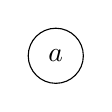
\begin{tikzpicture}
  \ARSnode{a};
\end{tikzpicture}

Normal forms: $a$. Terminating: True. Confluent: True. UNFs: True.

\paragraph{3.\; $A=\{a\},\; R=\{(a,a)\}$}
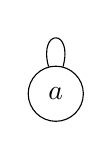
\begin{tikzpicture}
  \ARSnode{a};
  \path (a) edge[loop above] (a);
\end{tikzpicture}

Infinite sequence $a\to a\to\cdots$.  
Terminating: False. Confluent: True. UNFs: False.

\paragraph{4.\; $A=\{a,b,c\},\; R=\{(a,b),(a,c)\}$}
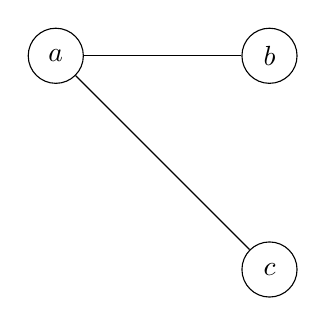
\begin{tikzpicture}[node distance=20mm]
  \ARSnode{a};
  \ARSnodeat{b}{right=of a}
  \ARSnodeat{c}{below=of b}
  \draw (a) edge (b) (a) edge (c);
\end{tikzpicture}

$b$ and $c$ are normal forms, so from $a$ two distinct endpoints are reachable.  
Terminating: True. Confluent: False. UNFs: False.

\paragraph{5.\; $A=\{a,b\},\; R=\{(a,a),(a,b)\}$}
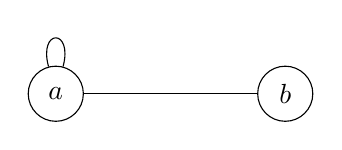
\begin{tikzpicture}[node distance=22mm]
  \ARSnode{a};
  \ARSnodeat{b}{right=of a}
  \draw (a) edge[loop above] (a) (a) edge (b);
\end{tikzpicture}

$b$ is normal; all paths from $a$ can reach $b$.  
Terminating: False. Confluent: True. UNFs: True.

\paragraph{6.\; $A=\{a,b,c\},\; R=\{(a,b),(b,b),(a,c)\}$}
\begin{tikzpicture}[node distance=22mm]
  \ARSnode{a};
  \ARSnodeat{b}{right=of a}
  \ARSnodeat{c}{below=of b}
  \draw (a) edge (b) (a) edge (c) (b) edge[loop above] (b);
\end{tikzpicture}

Non-terminating through $b\to b$; $c$ is normal but unreachable from $b$.  
Terminating: False. Confluent: False. UNFs: False.

\paragraph{7.\; $A=\{a,b,c\},\; R=\{(a,b),(b,b),(a,c),(c,c)\}$}
\begin{tikzpicture}[node distance=22mm]
  \ARSnode{a};
  \ARSnodeat{b}{right=of a}
  \ARSnodeat{c}{below=of b}
  \draw (a) edge (b) (a) edge (c) (b) edge[loop above] (b) (c) edge[loop right] (c);
\end{tikzpicture}

Both $b$ and $c$ loop indefinitely.  
Terminating: False. Confluent: False. UNFs: False.

\textbf{Summary Table:}
\begin{center}
\begin{tabular}{@{}clccc@{}}
\toprule
\# & $(A,R)$ & confluent & terminating & unique NFs \\
\midrule
1 & $(\varnothing,\varnothing)$ & True & True & True \\
2 & $(\{a\},\varnothing)$ & True & True & True \\
3 & $(\{a\},\{(a,a)\})$ & True & False & False \\
4 & $(\{a,b,c\},\{(a,b),(a,c)\})$ & False & True & False \\
5 & $(\{a,b\},\{(a,a),(a,b)\})$ & True & False & True \\
6 & $(\{a,b,c\},\{(a,b),(b,b),(a,c)\})$ & False & False & False \\
7 & $(\{a,b,c\},\{(a,b),(b,b),(a,c),(c,c)\})$ & False & False & False \\
\bottomrule
\end{tabular}
\end{center}

\textbf{All 8 Combinations:}
\begin{center}
\begin{tabular}{@{}ccccl@{}}
\toprule
confluent & terminating & unique NFs & example \\
\midrule
True  & True  & True  & ARS 2 (or 1) \\
True  & True  & False  & \textit{Impossible} \\
True  & False  & True  & ARS 5 \\
True  & False  & False  & ARS 3 \\
False & True  & True  & \textit{Impossible} \\
False & True  & False  & ARS 4 \\
False & False & True  & \textit{Impossible} \\
False & False & False & ARS 6 (or 7) \\
\bottomrule
\end{tabular}
\end{center}

\subsubsection{Questions}
\emph{Is there an easy way to tell from the graph if an ARS will terminate, or do you always have to trace every path?}

% ---------- Week 3 ----------
\subsection{Week 3}

\subsubsection{Notes and Exploration}
HW3 moved from drawing small ARS graphs to \textbf{string rewriting}. The key shift is that we are no longer just asking “what edges exist?”, but instead:
\begin{itemize}[leftmargin=1.4em]
  \item whether rewriting \emph{terminates} (i.e., there are no infinite $\to$-chains),
  \item what the \emph{normal forms} are (strings that cannot be rewritten further),
  \item and what the \emph{equivalence classes} are under $\leftrightarrow^{\!*}$ (the equality generated by rewriting).
\end{itemize}
The point is that $\leftrightarrow^{\!*}$ is the “real meaning” (what strings count as equal), while $\to$ is just one particular implementation.

\subsubsection{Homework}

\paragraph{Exercise 5.}
Rewrite rules over $\{a,b\}$:
\[
ab \to ba
\qquad
ba \to ab
\qquad
aa \to \varepsilon
\qquad
b \to \varepsilon
\]
(where $\varepsilon$ is the empty string).

\begin{enumerate}[label=\textbf{\arabic*.},leftmargin=1.6em]
  \item \textbf{Reduce some example strings (e.g.\ \texttt{abba} and \texttt{bababa}).}

  \textbf{Example 1:} \texttt{abba}.
  \[
  \texttt{abba} \to \texttt{aba} \to \texttt{aa} \to \varepsilon.
  \]
  So \texttt{abba} reduces to the normal form $\varepsilon$.

  \textbf{Example 2:} \texttt{bababa}.
  \[
  \texttt{bababa} \to \texttt{ababa} \to \texttt{aaba} \to \texttt{aaa} \to \texttt{a}.
  \]
  (One possible route: delete each $b$ using $b\to\varepsilon$, then reduce $aa\to\varepsilon$ once.)
  So \texttt{bababa} reduces to the normal form \texttt{a}.

  \item \textbf{Why is the ARS not terminating?}

  Because there is an infinite rewrite loop:
  \[
  \texttt{ab} \to \texttt{ba} \to \texttt{ab} \to \texttt{ba} \to \cdots
  \]
  So there exists an infinite $\to$-sequence, hence the system is \textbf{not terminating}.

  \item \textbf{Find two strings that are not equivalent. How many non-equivalent strings can you find?}

  Define an invariant:
  \[
  I(w) \;=\; (\#a\text{ in }w)\bmod 2.
  \]
  Check each rule preserves $I$:
  \begin{itemize}[leftmargin=1.4em]
    \item $ab\leftrightarrow ba$ does not change how many $a$'s appear.
    \item $aa \to \varepsilon$ changes the number of $a$'s by $-2$, so parity is unchanged.
    \item $b \to \varepsilon$ does not change the number of $a$'s.
  \end{itemize}
  Therefore $I(w)$ is constant on $\leftrightarrow^{\!*}$-equivalence classes.

  So $\varepsilon$ (even number of $a$'s) and \texttt{a} (odd number of $a$'s) are \textbf{not equivalent}.
  In fact, this shows there are \textbf{at least two} equivalence classes.

  \item \textbf{How many equivalence classes does $\leftrightarrow^{\!*}$ have? Describe them nicely. What are the normal forms?}

  The invariant above suggests exactly two classes:
  \begin{itemize}[leftmargin=1.4em]
    \item \textbf{Even-$a$ class:} all strings with an even number of $a$'s.
    \item \textbf{Odd-$a$ class:} all strings with an odd number of $a$'s.
  \end{itemize}

  \textbf{Why there are not more than two:}  
  From any string $w$, delete all $b$'s using $b\to\varepsilon$. This leaves a string $a^n$.  
  Then repeatedly apply $aa\to\varepsilon$:
  \[
  a^{2k} \to \varepsilon,
  \qquad
  a^{2k+1} \to a.
  \]
  So every string reduces to either $\varepsilon$ or \texttt{a}. These are irreducible (no rule applies), so they are \textbf{normal forms}.

  Therefore the normal forms are:
  \[
  \textbf{Normal forms: } \{\varepsilon,\; \texttt{a}\}.
  \]
  And the equivalence class is determined exactly by the parity of the number of $a$'s.

  \textbf{Specification (rule-free statement):} this system computes whether the number of $a$'s in the input string is \textbf{even or odd}.

  \item \textbf{Modify the ARS so it becomes terminating without changing its equivalence classes.}

  The nontermination comes from having \emph{both} swap directions. A terminating version is obtained by orienting the swap in only one direction, e.g.
  \[
  ba \to ab,
  \qquad
  aa \to \varepsilon,
  \qquad
  b \to \varepsilon.
  \]
  This is terminating because:
  \begin{itemize}[leftmargin=1.4em]
    \item each $ba\to ab$ decreases the number of “inversions” (a $b$ sitting to the left of an $a$),
    \item and $aa\to\varepsilon$, $b\to\varepsilon$ strictly decrease length.
  \end{itemize}
  The equivalence classes under $\leftrightarrow^{\!*}$ stay the same, because $\leftrightarrow^{\!*}$ already treats rules as reversible (it includes inverse steps), so allowing one swap direction is enough to generate the same notion of “same multiset up to swaps,” together with the same deletions/insertions of $aa$ and $b$.

  \item \textbf{Write down a question or two about strings that can be answered using the ARS.}

  Since the invariant is $(\#a)\bmod 2$, good “semantic” questions are:
  \begin{itemize}[leftmargin=1.4em]
    \item “Is this string equivalent to $\varepsilon$?” (i.e.\ does it have an even number of $a$'s?)
    \item “Are two strings equivalent?” (i.e.\ do they have the same parity of $a$'s?)
  \end{itemize}
\end{enumerate}

\bigskip
\paragraph{Exercise 5b.}
Same as Exercise 5, but replace $aa\to\varepsilon$ with $aa\to a$:
\[
ab \to ba
\qquad
ba \to ab
\qquad
aa \to a
\qquad
b \to \varepsilon
\]

\begin{enumerate}[label=\textbf{\arabic*.},leftmargin=1.6em]
  \item \textbf{Reduce the example strings again.}

  \textbf{Example 1:} \texttt{abba}.
  \[
  \texttt{abba} \to \texttt{aba} \to \texttt{aa} \to \texttt{a}.
  \]
  So the normal form is \texttt{a}.

  \textbf{Example 2:} \texttt{bababa}.
  Delete $b$'s to get \texttt{aaa}, then contract:
  \[
  \texttt{bababa} \to \texttt{aaa} \to \texttt{aa} \to \texttt{a}.
  \]
  So the normal form is again \texttt{a}.

  \item \textbf{Why is the ARS not terminating?}

  The same infinite loop still exists:
  \[
  \texttt{ab} \to \texttt{ba} \to \texttt{ab} \to \cdots
  \]
  Hence \textbf{not terminating}.

  \item \textbf{Find two strings that are not equivalent; how many non-equivalent strings can you find?}

  Here parity is \emph{not} invariant anymore, because $aa\to a$ changes $\#a$ by $-1$.

  A correct invariant is:
  \[
  J(w) \;=\; \text{“does $w$ contain at least one $a$?”}
  \]
  Check:
  \begin{itemize}[leftmargin=1.4em]
    \item swaps do not create/destroy $a$'s,
    \item $b\to\varepsilon$ does not affect whether an $a$ exists,
    \item $aa\to a$ never removes the \emph{last} $a$ (it turns two $a$'s into one $a$).
  \end{itemize}
  So “having an $a$” is invariant under $\leftrightarrow^{\!*}$.

  Therefore $\varepsilon$ (no $a$) and \texttt{a} (has an $a$) are \textbf{not equivalent}, so there are at least two equivalence classes.

  \item \textbf{How many equivalence classes are there? What are the normal forms?}

  Every string either has no $a$ (only $b$'s), or has at least one $a$.
  \begin{itemize}[leftmargin=1.4em]
    \item If $w$ has no $a$, then repeatedly delete $b$'s to reach $\varepsilon$.
    \item If $w$ has at least one $a$, delete all $b$'s, leaving $a^n$ with $n\ge 1$, then repeatedly apply $aa\to a$ until only \texttt{a} remains.
  \end{itemize}
  So again the normal forms are:
  \[
  \textbf{Normal forms: } \{\varepsilon,\; \texttt{a}\}.
  \]
  But now they represent two different meanings:
  \begin{itemize}[leftmargin=1.4em]
    \item $\varepsilon$ = “there are no $a$'s in the input,”
    \item \texttt{a} = “there is at least one $a$ in the input.”
  \end{itemize}

  \textbf{Specification (rule-free statement):} this system computes whether the input string contains an $a$ or not.

  \item \textbf{Modify the ARS to become terminating without changing equivalence classes.}

  As before, orient the swap one way:
  \[
  ba \to ab,
  \qquad
  aa \to a,
  \qquad
  b \to \varepsilon.
  \]
  Termination follows from the same measure idea (inversions decrease under $ba\to ab$ and length decreases under $aa\to a$ and $b\to\varepsilon$), while $\leftrightarrow^{\!*}$-equivalence remains the same.

  \item \textbf{Questions answerable using the ARS.}

  Since the invariant is “has an $a$,” natural questions are:
  \begin{itemize}[leftmargin=1.4em]
    \item “Is this string equivalent to $\varepsilon$?” (i.e.\ does it have no $a$?)
    \item “Are two strings equivalent?” (i.e.\ do they either both have an $a$, or both have none?)
  \end{itemize}
\end{enumerate}

\subsubsection{Questions}
\emph{Could we make a version of 5b that is still non-terminating but somehow keeps unique normal forms?}

% ---------- Week 4 ----------
\subsection{Week 4}

\subsubsection{Notes and Exploration}
This week we focused on \textbf{termination proofs} using \textbf{measure functions}.
The general pattern is:
\begin{itemize}[leftmargin=1.4em]
  \item pick a function $\varphi(\text{state})$ that maps every program state to a value in a well-founded set (usually $\mathbb{N}$),
  \item show $\varphi$ is always $\ge 0$ (so it cannot decrease forever), and
  \item show every loop iteration (or recursive call) makes $\varphi$ strictly smaller.
\end{itemize}
If both are true, then an infinite execution would force an infinite strictly-decreasing sequence in $\mathbb{N}$, which is impossible. So the program must terminate.

\subsubsection{Homework}

\paragraph{HW 4.1 (Euclidean Algorithm).}
\textbf{Algorithm.}
\begin{verbatim}
while b != 0:
  temp = b
  b = a mod b
  a = temp
return a
\end{verbatim}

\textbf{Question: Under what conditions does this always terminate?}

A clean set of conditions is:
\[
a,b \in \mathbb{N} \quad \text{(natural numbers),}
\]
and we interpret $a \bmod b$ in the standard way when $b>0$, meaning:
\[
0 \le (a \bmod b) < b.
\]
(Also note: if $b=0$ at the start, the loop does zero iterations and the algorithm terminates immediately.)

\textbf{Measure function.}
Define the measure on program states $(a,b)$ by
\[
\varphi(a,b) = b.
\]

\textbf{Proof of termination.}
Assume we are in a loop iteration, so the guard is true and therefore $b \ne 0$, i.e.\ $b>0$ in $\mathbb{N}$.

Inside the loop we assign
\[
b \;:=\; a \bmod b.
\]
By the defining property of the remainder when $b>0$,
\[
0 \le a \bmod b < b.
\]
So after the assignment, the new value of $b$ (call it $b'$) satisfies:
\[
0 \le b' < b.
\]
That means the measure strictly decreases each iteration:
\[
\varphi(a',b') = b' < b = \varphi(a,b).
\]

Also, $\varphi(a,b)=b$ is always a natural number, so it is bounded below by $0$ and cannot decrease forever.
Therefore the loop can only run finitely many times, so the algorithm terminates.

\textbf{Conclusion.}
Under the condition that $a,b\in\mathbb{N}$ and $\bmod$ is the standard remainder operation (so $0\le a\bmod b < b$ for $b>0$), the algorithm always terminates.

\bigskip

\paragraph{HW 4.2 (Merge Sort Fragment).}
\textbf{Code fragment.}
\begin{verbatim}
function merge_sort(arr, left, right):
  if left >= right:
    return
  mid = (left + right) / 2
  merge_sort(arr, left, mid)
  merge_sort(arr, mid+1, right)
  merge(arr, left, mid, right)
\end{verbatim}

\textbf{Claim.} The function
\[
\varphi(left,right) = right - left + 1
\]
is a measure function for \texttt{merge\_sort}.

\textbf{Why this is a valid measure.}
When \texttt{merge\_sort} actually recurses, it is in the case $left < right$ (since if $left \ge right$ it returns immediately).
So in the recursive case we have $right-left \ge 1$, which implies:
\[
\varphi(left,right) = right-left+1 \ge 2.
\]
In particular, $\varphi(left,right)\in\mathbb{N}$ and is always at least $1$ when $left \le right$.

\textbf{Strict decrease on recursive calls.}
Let
\[
n = \varphi(left,right)=right-left+1.
\]
In the recursive case $n\ge 2$. The midpoint $mid$ is chosen so that
\[
left \le mid < right.
\]
Now compare the measures.

\emph{First recursive call:} \texttt{merge\_sort(arr,left,mid)} has measure
\[
\varphi(left,mid) = mid-left+1.
\]
Because $mid<right$, we have $mid-left+1 \le (right-1)-left+1 = right-left = n-1$.
So
\[
\varphi(left,mid) \le n-1 < n.
\]

\emph{Second recursive call:} \texttt{merge\_sort(arr,mid+1,right)} has measure
\[
\varphi(mid+1,right) = right-(mid+1)+1 = right-mid.
\]
Because $left \le mid$, we have $right-mid \le right-left = n-1$.
So
\[
\varphi(mid+1,right) \le n-1 < n.
\]

Thus, in both recursive calls, the measure is strictly smaller than the original $n$.

\textbf{Bounded below.}
The measure $\varphi$ always takes values in $\mathbb{N}$ and (for any non-empty interval) is at least $1$.
So it cannot decrease infinitely many times.

\textbf{Conclusion.}
Every recursive call strictly decreases $\varphi(left,right)=right-left+1$, and the measure is bounded below in $\mathbb{N}$, so the recursion must terminate.

\subsubsection{Questions}
\emph{When picking a measure function, how do I decide whether to measure “size of the input” (like $right-left+1$) versus something more indirect (like number of inversions or a lexicographic pair of measures)?}


% ---------- Week 5 ----------
\subsection{Week 5}

\subsubsection{Notes and Exploration}
This week we practiced $\lambda$-calculus reduction using:
\begin{itemize}
  \item \textbf{$\alpha$-renaming} (renaming bound variables) to avoid confusion/capture.
  \item \textbf{$\beta$-reduction}: $(\lambda x.\,M)\,N \mapsto M[N/x]$ (substitute $N$ for free occurrences of $x$ in $M$).
\end{itemize}

\subsubsection{Homework}
Evaluate:
\[
(\lambda f.\lambda x.f(f(x)))\,(\lambda f.\lambda x.f(f(f(x)))).
\]

Let
\[
A := \lambda f.\lambda x.\, f(f(x))
\qquad\text{and}\qquad
B := \lambda f.\lambda x.\, f(f(f(x))).
\]
We compute \(A\,B\).

\medskip
\textbf{Step 1 (\(\beta\)-reduction).}
\[
(\lambda f.\lambda x.\, f(f(x)))\,B
\;\mapsto_{\beta}\;
\lambda x.\, B(B(x)).
\]
So it remains to reduce \(B(B(x))\).

\medskip
\textbf{Step 2 (reduce \(B(x)\)).}
\[
B(x)
=
(\lambda f.\lambda x.\, f(f(f(x))))\,x.
\]
To avoid confusion with two different binders named \(x\), rename the inner bound variable \(x\) to \(u\) (\(\alpha\)-conversion):
\[
(\lambda f.\lambda u.\, f(f(f(u))))\,x
\;\mapsto_{\beta}\;
\lambda u.\, x(x(x(u))).
\]
Call this result
\[
G := \lambda u.\, x(x(x(u))).
\]
So \(B(x) \mapsto G\).

\medskip
\textbf{Step 3 (now reduce \(B(G)\)).}
\[
B(G)
=
(\lambda f.\lambda x.\, f(f(f(x))))\,G
\;\mapsto_{\beta}\;
\lambda x.\, G(G(G(x))).
\]
Again rename the bound variable \(x\) to \(y\) to keep symbols distinct:
\[
B(G) \mapsto \lambda y.\, G(G(G(y))).
\]

\medskip
\textbf{Step 4 (expand what \(G\) does).}
Recall \(G(t) = x(x(x(t)))\). Then:
\[
G(y) = x^3(y),
\]
\[
G(G(y)) = G(x^3(y)) = x^3(x^3(y)) = x^6(y),
\]
\[
G(G(G(y))) = G(x^6(y)) = x^3(x^6(y)) = x^9(y).
\]
So
\[
\lambda y.\, G(G(G(y))) \;=\; \lambda y.\, x^9(y).
\]

\medskip
\textbf{Final answer.}
Putting this back into Step 1:
\[
A\,B \;\mapsto\; \lambda x.\, B(B(x))
\;\mapsto\; \lambda x.\, (\lambda y.\, x^9(y)).
\]
Equivalently, this is a function that takes \(x\) and returns the function \(y \mapsto x^9(y)\).

\subsubsection{Questions}
\emph{What would happen if we swapped the two functions in the workout?}

% ---------- Week 6 ----------
\subsection{Week 6}

\subsubsection{Notes and Exploration}
We computed factorial using the fixed-point combinator \texttt{fix}, and we practiced reducing
\texttt{let rec} by rewriting it into \texttt{fix} and then applying \(\beta\)-reduction step by step.

\subsubsection{Homework}
Compute:
\[
\texttt{let rec fact = \textbackslash n.\ if n=0 then 1 else n * fact (n-1) in fact 3}.
\]

We use the computation rules:
\[
\texttt{fix F} \mapsto \texttt{F (fix F)}, \qquad
\texttt{let x = e1 in e2} \mapsto (\lambda x.\,e2)\,e1,
\]
\[
\texttt{let rec f = e1 in e2} \mapsto \texttt{let f = (fix (\textbackslash f.\,e1)) in e2}.
\]
We also use the given computation rules for \texttt{if}, equality with \(0\), and basic arithmetic
(e.g. \(3=0\mapsto \texttt{False}\), \(0=0\mapsto \texttt{True}\), \(\texttt{if True then A else B}\mapsto A\),
\(\texttt{if False then A else B}\mapsto B\), and \(3-1\mapsto 2\), etc.).

\medskip
\noindent
Let
\[
F \;:=\; (\lambda \texttt{fact}.\ \lambda n.\ \texttt{if } n=0 \texttt{ then } 1 \texttt{ else } n * \texttt{fact}(n-1)).
\]

\medskip
\noindent\textbf{Start:}
\[
E_0 \;:=\; \texttt{let rec fact = \textbackslash n.\ if n=0 then 1 else n * fact (n-1) in fact 3}.
\]

\medskip
\noindent\textbf{Step-by-step reduction:}
\begin{align*}
E_0
&\mapsto \texttt{let fact = (fix (\textbackslash fact.\ \textbackslash n.\ if n=0 then 1 else n * fact (n-1))) in fact 3}
&&\langle \text{def of let rec} \rangle \\[4pt]
&\mapsto (\lambda \texttt{fact}.\ \texttt{fact}\ 3)\ (\texttt{fix }F)
&&\langle \text{def of let} \rangle \\[4pt]
&\mapsto (\texttt{fix }F)\ 3
&&\langle \beta \rangle \\[8pt]
&\mapsto (F(\texttt{fix }F))\ 3
&&\langle \text{def of fix} \rangle \\[4pt]
&\mapsto (\lambda n.\ \texttt{if } n=0 \texttt{ then } 1 \texttt{ else } n * (\texttt{fix }F)(n-1))\ 3
&&\langle \beta \rangle \\[4pt]
&\mapsto \texttt{if } 3=0 \texttt{ then } 1 \texttt{ else } 3 * (\texttt{fix }F)(3-1)
&&\langle \beta \rangle \\[4pt]
&\mapsto \texttt{if False then } 1 \texttt{ else } 3 * (\texttt{fix }F)(3-1)
&&\langle \text{def of } (=0) \rangle \\[4pt]
&\mapsto 3 * (\texttt{fix }F)(3-1)
&&\langle \text{def of if} \rangle \\[4pt]
&\mapsto 3 * (\texttt{fix }F)\ 2
&&\langle \text{arith: }3-1\mapsto 2 \rangle \\[10pt]
&\mapsto 3 * (F(\texttt{fix }F))\ 2
&&\langle \text{def of fix} \rangle \\[4pt]
&\mapsto 3 * (\lambda n.\ \texttt{if } n=0 \texttt{ then } 1 \texttt{ else } n * (\texttt{fix }F)(n-1))\ 2
&&\langle \beta \rangle \\[4pt]
&\mapsto 3 * (\texttt{if } 2=0 \texttt{ then } 1 \texttt{ else } 2 * (\texttt{fix }F)(2-1))
&&\langle \beta \rangle \\[4pt]
&\mapsto 3 * (\texttt{if False then } 1 \texttt{ else } 2 * (\texttt{fix }F)(2-1))
&&\langle \text{def of } (=0) \rangle \\[4pt]
&\mapsto 3 * (2 * (\texttt{fix }F)(2-1))
&&\langle \text{def of if} \rangle \\[4pt]
&\mapsto 3 * (2 * (\texttt{fix }F)\ 1)
&&\langle \text{arith: }2-1\mapsto 1 \rangle \\[10pt]
&\mapsto 3 * (2 * (F(\texttt{fix }F))\ 1)
&&\langle \text{def of fix} \rangle \\[4pt]
&\mapsto 3 * (2 * (\lambda n.\ \texttt{if } n=0 \texttt{ then } 1 \texttt{ else } n * (\texttt{fix }F)(n-1))\ 1)
&&\langle \beta \rangle \\[4pt]
&\mapsto 3 * (2 * (\texttt{if } 1=0 \texttt{ then } 1 \texttt{ else } 1 * (\texttt{fix }F)(1-1)))
&&\langle \beta \rangle \\[4pt]
&\mapsto 3 * (2 * (\texttt{if False then } 1 \texttt{ else } 1 * (\texttt{fix }F)(1-1)))
&&\langle \text{def of } (=0) \rangle \\[4pt]
&\mapsto 3 * (2 * (1 * (\texttt{fix }F)(1-1)))
&&\langle \text{def of if} \rangle \\[4pt]
&\mapsto 3 * (2 * (1 * (\texttt{fix }F)\ 0))
&&\langle \text{arith: }1-1\mapsto 0 \rangle \\[10pt]
&\mapsto 3 * (2 * (1 * (F(\texttt{fix }F))\ 0))
&&\langle \text{def of fix} \rangle \\[4pt]
&\mapsto 3 * (2 * (1 * (\lambda n.\ \texttt{if } n=0 \texttt{ then } 1 \texttt{ else } n * (\texttt{fix }F)(n-1))\ 0))
&&\langle \beta \rangle \\[4pt]
&\mapsto 3 * (2 * (1 * (\texttt{if } 0=0 \texttt{ then } 1 \texttt{ else } 0 * (\texttt{fix }F)(0-1))))
&&\langle \beta \rangle \\[4pt]
&\mapsto 3 * (2 * (1 * (\texttt{if True then } 1 \texttt{ else } 0 * (\texttt{fix }F)(0-1))))
&&\langle \text{def of } (=0) \rangle \\[4pt]
&\mapsto 3 * (2 * (1 * 1))
&&\langle \text{def of if} \rangle \\[8pt]
&\mapsto 3 * (2 * 1)
&&\langle \text{arith: }1*1\mapsto 1 \rangle \\[4pt]
&\mapsto 3 * 2
&&\langle \text{arith: }2*1\mapsto 2 \rangle \\[4pt]
&\mapsto 6
&&\langle \text{arith: }3*2\mapsto 6 \rangle
\end{align*}

\textbf{Conclusion.} \\
By repeatedly expanding \texttt{fix} (to unfold recursion) and then applying \(\beta\)-reduction and the
\texttt{if}/arithmetic rules, the term reduces to \(\mathbf{6}\). So \(\texttt{fact 3}\) computes \(3!\).

\subsubsection{Questions}
\emph{Would using $\alpha$-conversion anywhere in this computation change the result, or just make it cleaner?}


% ---------- Week 7 ----------
\subsection{Week 7}

\subsubsection{Notes and Exploration}
Parsing and context-free grammars. We use the grammar (nonterminals \texttt{Exp}, \texttt{Exp1}, \texttt{Exp2}, and \texttt{Int}):

\begin{verbatim}
Exp  -> Exp '+' Exp1
Exp  -> Exp1
Exp1 -> Exp1 '*' Exp2
Exp1 -> Exp2
Exp2 -> Int
Exp2 -> '(' Exp ')'
Int  -> 0 | 1 | 2 | 3 | 4 | 5 | 6 | 7 | 8 | 9
\end{verbatim}

\subsubsection{Homework: Parse Trees}
Below are derivation trees (concrete syntax trees) for the required expressions.
Nonterminals are boxed; terminals are leaves.
(\textbf{Note:} Integers are introduced using the \texttt{Int}-rule, i.e.\ \texttt{Exp2 -> Int -> digit}.)

% ---------------------------------------------------------
\paragraph{(a) \texttt{2+1}}
\begin{center}
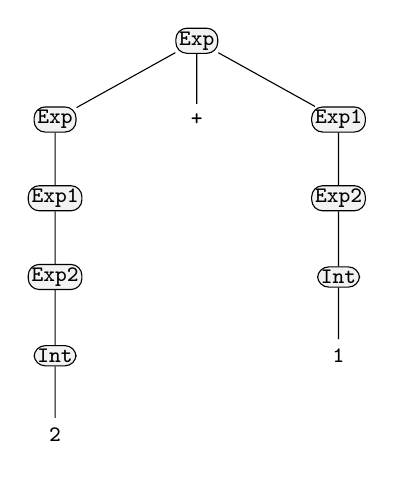
\begin{tikzpicture}[ptree]
\node[nt]{Exp}
  child { node[nt]{Exp}
    child { node[nt]{Exp1}
      child { node[nt]{Exp2}
        child { node[nt]{Int}
          child { node[tm]{2} }
        }
      }
    }
  }
  child { node[tm]{+} }
  child { node[nt]{Exp1}
    child { node[nt]{Exp2}
      child { node[nt]{Int}
        child { node[tm]{1} }
      }
    }
  };
\end{tikzpicture}
\end{center}

% ---------------------------------------------------------
\paragraph{(b) \texttt{1+2*3}}
\begin{center}
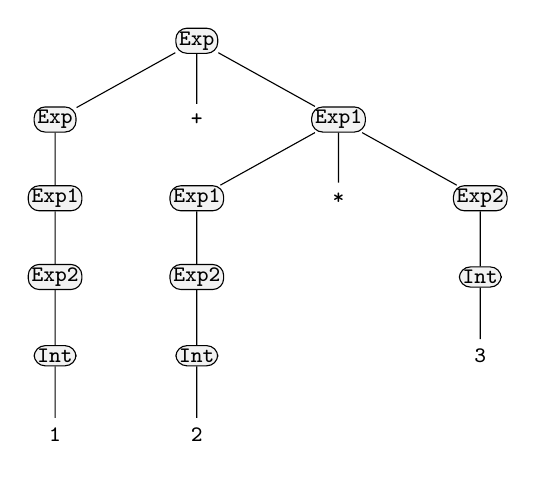
\begin{tikzpicture}[ptree]
\node[nt]{Exp}
  child { node[nt]{Exp}
    child { node[nt]{Exp1}
      child { node[nt]{Exp2}
        child { node[nt]{Int}
          child { node[tm]{1} }
        }
      }
    }
  }
  child { node[tm]{+} }
  child { node[nt]{Exp1}
    child { node[nt]{Exp1}
      child { node[nt]{Exp2}
        child { node[nt]{Int}
          child { node[tm]{2} }
        }
      }
    }
    child { node[tm]{*} }
    child { node[nt]{Exp2}
      child { node[nt]{Int}
        child { node[tm]{3} }
      }
    }
  };
\end{tikzpicture}
\end{center}

% ---------------------------------------------------------
\paragraph{(c) \texttt{1+(2*3)}}
\begin{center}
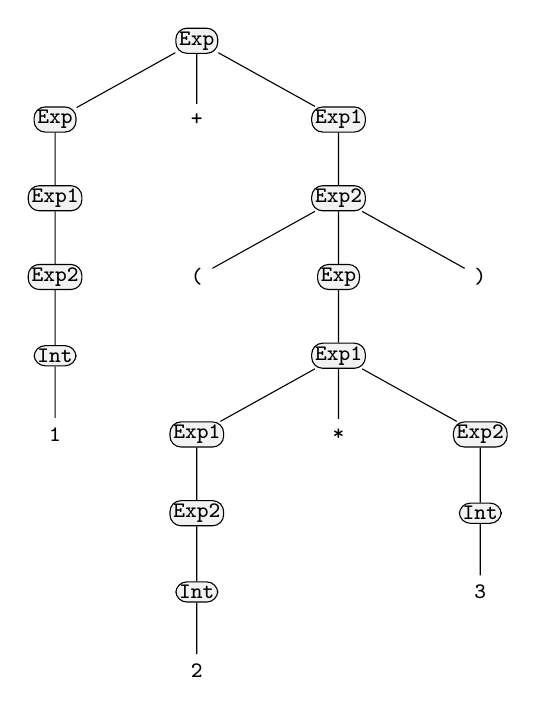
\begin{tikzpicture}[ptree]
\node[nt]{Exp}
  child { node[nt]{Exp}
    child { node[nt]{Exp1}
      child { node[nt]{Exp2}
        child { node[nt]{Int}
          child { node[tm]{1} }
        }
      }
    }
  }
  child { node[tm]{+} }
  child { node[nt]{Exp1}
    child { node[nt]{Exp2}
      child { node[tm]{(} }
      child { node[nt]{Exp}
        child { node[nt]{Exp1}
          child { node[nt]{Exp1}
            child { node[nt]{Exp2}
              child { node[nt]{Int}
                child { node[tm]{2} }
              }
            }
          }
          child { node[tm]{*} }
          child { node[nt]{Exp2}
            child { node[nt]{Int}
              child { node[tm]{3} }
            }
          }
        }
      }
      child { node[tm]{)} }
    }
  };
\end{tikzpicture}
\end{center}

% ---------------------------------------------------------
\paragraph{(d) \texttt{(1+2)*3}}
\begin{center}
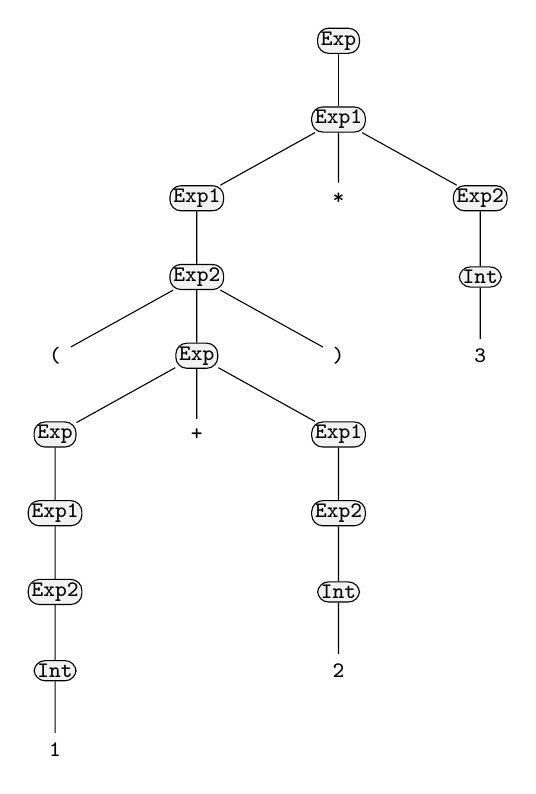
\begin{tikzpicture}[ptree]
\node[nt]{Exp}
  child { node[nt]{Exp1}
    child { node[nt]{Exp1}
      child { node[nt]{Exp2}
        child { node[tm]{(} }
        child { node[nt]{Exp}
          child { node[nt]{Exp}
            child { node[nt]{Exp1}
              child { node[nt]{Exp2}
                child { node[nt]{Int}
                  child { node[tm]{1} }
                }
              }
            }
          }
          child { node[tm]{+} }
          child { node[nt]{Exp1}
            child { node[nt]{Exp2}
              child { node[nt]{Int}
                child { node[tm]{2} }
              }
            }
          }
        }
        child { node[tm]{)} }
      }
    }
    child { node[tm]{*} }
    child { node[nt]{Exp2}
      child { node[nt]{Int}
        child { node[tm]{3} }
      }
    }
  };
\end{tikzpicture}
\end{center}

% ---------------------------------------------------------
\paragraph{(e) \texttt{1+2*3+4*5+6}}
\begin{center}
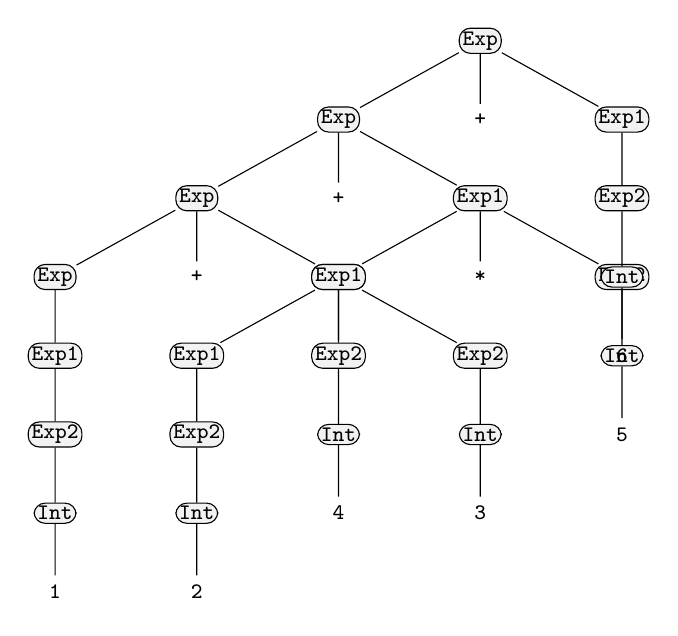
\begin{tikzpicture}[ptree]
\node[nt]{Exp}
  % left part: (1 + 2*3) + 4*5
  child { node[nt]{Exp}
    child { node[nt]{Exp}
      % 1 + 2*3
      child { node[nt]{Exp}
        child { node[nt]{Exp1}
          child { node[nt]{Exp2}
            child { node[nt]{Int}
              child { node[tm]{1} }
            }
          }
        }
      }
      child { node[tm]{+} }
      child { node[nt]{Exp1}
        child { node[nt]{Exp1}
          child { node[nt]{Exp2}
            child { node[nt]{Int}
              child { node[tm]{2} }
            }
          }
        }
        child { node[tm]{*} }
        child { node[nt]{Exp2}
          child { node[nt]{Int}
            child { node[tm]{3} }
          }
        }
      }
    }
    child { node[tm]{+} }
    % 4*5
    child { node[nt]{Exp1}
      child { node[nt]{Exp1}
        child { node[nt]{Exp2}
          child { node[nt]{Int}
            child { node[tm]{4} }
          }
        }
      }
      child { node[tm]{*} }
      child { node[nt]{Exp2}
        child { node[nt]{Int}
          child { node[tm]{5} }
        }
      }
    }
  }
  child { node[tm]{+} }
  % + 6
  child { node[nt]{Exp1}
    child { node[nt]{Exp2}
      child { node[nt]{Int}
        child { node[tm]{6} }
      }
    }
  };
\end{tikzpicture}
\end{center}

% =========================================================
\subsubsection{Questions}
\emph{Could this grammar still work if “+” and “*” had the same priority?}


% ---------- Week 8 ----------
\subsection{Week 8}

\subsubsection{Notes and Exploration}
I completed Levels 5--8 of the \emph{Natural Number Game} (NNG). The key tools were:
\begin{itemize}[leftmargin=1.4em]
  \item \textbf{Rewriting} with \texttt{rw [lemma]} to substitute equals for equals.
  \item \textbf{\texttt{rfl}} to close a goal when both sides are definitionally identical.
  \item Peano-style equations for addition and numerals, including \texttt{add\_zero}, \texttt{add\_succ}, \texttt{add\_one}, \texttt{one\_eq\_succ\_zero}, and \texttt{two\_eq\_succ\_one}.
\end{itemize}

\subsubsection{Homework (NNG Levels 5--8)}
\paragraph{5/8: Adding zero.} \emph{Goal:} $a + (b+0) + (c+0) = a+b+c$.\\
\emph{Lean steps:} \texttt{rw [add\_zero]} (on $b+0$), \texttt{rw [add\_zero]} (on $c+0$), \texttt{rfl}.

\paragraph{6/8: Precision rewriting.} \emph{Goal:} $a + (b+0) + (c+0) = a+b+c$.\\
\emph{Lean steps:} \texttt{rw [add\_zero]} (on $b+0$), \texttt{rw [add\_zero]} (on $c+0$), \texttt{rfl}.

\paragraph{7/8: \texttt{add\_succ}.} \emph{Goal:} $\mathrm{succ}\,n = n+1$.\\
\emph{Lean steps:} \texttt{rw [one\_eq\_succ\_zero]} to get $n+1=n+\mathrm{succ}\,0$; \texttt{rw [add\_succ]} to obtain $\mathrm{succ}(n+0)$; \texttt{rw [add\_zero]}; \texttt{rfl}.

\paragraph{8/8: $2+2=4$.} \emph{Outline:} Rewrite $2$ and $4$ as successors (\texttt{two\_eq\_succ\_one}, etc.), use \texttt{add\_succ} to pull \(\mathrm{succ}\) out of addition stepwise, and finish by \texttt{rfl} once both sides match.

\subsubsection{Natural-Language Proof (English math proof)}
\paragraph{Claim.} \(2+2=4\).

\paragraph{Assumptions/Definitions.}
Let \(0\) be the base natural number and \(\mathrm{succ}(n)\) the successor of \(n\).
Define \(1=\mathrm{succ}(0)\), \(2=\mathrm{succ}(1)\), and \(4=\mathrm{succ}(\mathrm{succ}(\mathrm{succ}(\mathrm{succ}(0))))\).
Addition is defined by the Peano axioms:
\[
\forall a,\; a+0=a \quad\text{and}\quad \forall a,b,\; a+\mathrm{succ}(b)=\mathrm{succ}(a+b).
\]

\paragraph{Proof.}
We compute \(2+2\) using the addition axioms.
First rewrite \(2=\mathrm{succ}(1)\), so
\[
2+2 \;=\; 2+\mathrm{succ}(1) \;=\; \mathrm{succ}(2+1) \quad\text{(by the second axiom).}
\]
Again rewrite \(1=\mathrm{succ}(0)\) to get
\[
2+1 \;=\; 2+\mathrm{succ}(0) \;=\; \mathrm{succ}(2+0) \;=\; \mathrm{succ}(2) \quad\text{(using both axioms).}
\]
Therefore
\[
2+2 \;=\; \mathrm{succ}(2+1) \;=\; \mathrm{succ}(\mathrm{succ}(2)).
\]
Since \(2=\mathrm{succ}(1)\), we have
\[
\mathrm{succ}(\mathrm{succ}(2))=\mathrm{succ}(\mathrm{succ}(\mathrm{succ}(1)))=
\mathrm{succ}(\mathrm{succ}(\mathrm{succ}(\mathrm{succ}(0))))=4.
\]
Hence \(2+2=4\). \(\square\)

\subsubsection{Discord Question}
\emph{When using \texttt{rw [add\_zero]}, how does Lean know which part of the equation to rewrite first?}

% ---------- Week 9 ----------
\subsection{Week 9}

\subsubsection{Notes and Exploration}
This week I worked through \emph{Addition World} in the Natural Number Game.  
Key theorems proved in this world:
\begin{itemize}[leftmargin=1.4em]
  \item \textbf{zero\_add:} $0 + n = n$ (proved by induction).
  \item \textbf{succ\_add:} $\mathrm{succ}(a) + b = \mathrm{succ}(a + b)$ (proved by induction).
  \item \textbf{add\_comm:} $a + b = b + a$ (commutativity of $+$).
  \item \textbf{add\_assoc:} $(a + b) + c = a + (b + c)$ (associativity of $+$).
  \item \textbf{add\_right\_comm:} $(a + b) + c = (a + c) + b$.
\end{itemize}

The HW 9 instruction is:  
For Level 5 of addition world (\texttt{add\_right\_comm}), give two solutions in the report:
(1) a proof that uses induction and  
(2) a proof that does \emph{not} use induction.  
For each version, also write the corresponding ``pen-and-paper'' math proof.

\subsubsection{Homework (Addition World Level 5 / HW 9)}

\paragraph{Theorem (Level 5).}
For all natural numbers $a,b,c$, we have
\[
(a + b) + c \;=\; (a + c) + b.
\]
In Lean, this theorem is called \texttt{add\_right\_comm}.

\bigskip
\noindent\textbf{Solution A: With Induction.}  
We prove \texttt{add\_right\_comm} by induction on $c$.

\emph{Lean tactic steps:}
\begin{itemize}[leftmargin=1.4em]
  \item \texttt{induction c with d hd}
  \item \texttt{rw [add\_zero]}
  \item \texttt{rw [add\_zero]}
  \item \texttt{rfl}
  \item \texttt{rw [add\_succ]}
  \item \texttt{rw [succ\_add]}
  \item \texttt{rw [hd]}
  \item \texttt{rfl}
\end{itemize}

Explanation of structure (what the tactics are doing, summarized in math terms):

\emph{Base case ($c=0$).}  
Goal:
\[
(a+b)+0 \;=\; (a+0)+b.
\]
By \texttt{add\_zero}, $(a+b)+0 = a+b$, and $(a+0)+b = a+b$.  
So both sides are $a+b$. Closed by \texttt{rfl}.

\emph{Inductive step ($c = \mathrm{succ}(d)$).}  
Induction hypothesis (called \texttt{hd} in Lean):
\[
(a+b)+d \;=\; (a+d)+b.
\]
Goal:
\[
(a+b)+\mathrm{succ}(d) \;=\; (a+\mathrm{succ}(d))+b.
\]

Using the Peano definition of $+$ on the right argument,
\[
(a+b)+\mathrm{succ}(d) = \mathrm{succ}((a+b)+d)
\quad\text{and}\quad
a+\mathrm{succ}(d) = \mathrm{succ}(a+d).
\]
So the right-hand side becomes
\[
(a+\mathrm{succ}(d))+b
= (\mathrm{succ}(a+d))+b
= \mathrm{succ}\big((a+d)+b\big)
\]
using \texttt{succ\_add}, which says $\mathrm{succ}(x)+y=\mathrm{succ}(x+y)$.

Thus the goal reduces to
\[
\mathrm{succ}\big((a+b)+d\big)
=
\mathrm{succ}\big((a+d)+b\big).
\]
By the induction hypothesis, $(a+b)+d = (a+d)+b$, so the two $\mathrm{succ}(\cdot)$ terms are equal. This closes with \texttt{rfl}.

\emph{Conclusion.}  
By induction on $c$, $(a+b)+c = (a+c)+b$ holds for all $a,b,c$.

\bigskip
\noindent\textbf{Solution B: Without Induction.}  
We can also prove \texttt{add\_right\_comm} using only associativity and commutativity of addition, without \texttt{induction}.

\emph{Lean tactic steps (no induction):}
\begin{itemize}[leftmargin=1.4em]
  \item \texttt{rw [add\_assoc]}
  \item \texttt{rw [add\_comm b c]}
  \item \texttt{rw [\textbackslash leftarrow{} add\_assoc]}
  \item \texttt{rfl}
\end{itemize}

Those steps correspond exactly to the following algebra moves:
\[
(a+b)+c
\;=\;
a+(b+c)
\quad\text{(associativity, \texttt{add\_assoc})}
\]
\[
=\;
a+(c+b)
\quad\text{(commutativity on $b+c$, \texttt{add\_comm b c})}
\]
\[
=\;
(a+c)+b
\quad\text{(associativity again, undoing \texttt{add\_assoc})}.
\]
This matches the goal $(a+b)+c = (a+c)+b$.

\bigskip
\noindent\textbf{English/Pen-and-Paper Proofs for HW 9}

\paragraph{Solution A (Induction Proof in Math).}
We prove $(a+b)+c = (a+c)+b$ for all $a,b,c \in \mathbb{N}$ by induction on $c$.

\textbf{Base case:} $c=0$.  
Then
\[
(a+b)+0 = a+b
\quad\text{and}\quad
(a+0)+b = a+b,
\]
because $x+0=x$ for any $x$.  
So $(a+b)+0 = (a+0)+b$.

\textbf{Inductive step:} Assume $(a+b)+d = (a+d)+b$ for some $d$.  
We must show $(a+b)+\mathrm{succ}(d) = (a+\mathrm{succ}(d))+b$.

By the Peano definition of addition on the right argument,
\[
(a+b)+\mathrm{succ}(d) = \mathrm{succ}((a+b)+d).
\]
Also,
\[
a+\mathrm{succ}(d) = \mathrm{succ}(a+d),
\]
so
\[
(a+\mathrm{succ}(d))+b 
= (\mathrm{succ}(a+d))+b 
= \mathrm{succ}((a+d)+b),
\]
using the lemma $\mathrm{succ}(x)+y = \mathrm{succ}(x+y)$.

So it suffices to show
\[
\mathrm{succ}((a+b)+d) = \mathrm{succ}((a+d)+b),
\]
which follows from the induction hypothesis $(a+b)+d = (a+d)+b$.  
Therefore the statement holds for $\mathrm{succ}(d)$.

By induction on $c$, $(a+b)+c = (a+c)+b$ for all $a,b,c$.

\paragraph{Solution B (Algebraic / No Induction).}
We use associativity and commutativity of addition on $\mathbb{N}$.

Starting from the left-hand side,
\[
(a+b)+c = a+(b+c)
\quad\text{(associativity of $+$)},
\]
\[
= a+(c+b)
\quad\text{(commutativity of $+$)},
\]
\[
= (a+c)+b
\quad\text{(associativity of $+$ again)}.
\]
This is exactly the desired right-hand side $(a+c)+b$.  
No induction was needed.

\subsubsection{Questions}
\emph{When should I solve these problems using induction vs without?}

% ---------- Week 10 ----------
\subsection{Week 10}

\subsubsection{Notes and Exploration}
This week I finished the \textbf{Lean Logic Game} tutorial on implications, called \emph{Party Snacks}. The tutorial shows that
\begin{itemize}[leftmargin=1.4em]
  \item an implication $P \to Q$ is a function from evidence of $P$ to evidence of $Q$;
  \item conjunction $P \land Q$ is a pair made with \texttt{and\_intro};
  \item taking a function of \emph{two} inputs and turning it into a function of \emph{one} input that returns a function (currying) is exactly what Lean is doing when we write \texttt{fun x => fun y => ...}.
\end{itemize}
Levels 6--9 are the ones required for the HW, so below I spell out every little step.

\subsubsection{Homework (Party Snacks, Levels 6--9)}

% ---------------- Level 6 ----------------
\paragraph{Level 6/9 (\texttt{and\_imp}).}
\textbf{Goal.} Build
\[
C \to D \to S
\]
from the assumption
\[
h : C \land D \to S.
\]

So Lean is asking us to produce a \emph{function} that, when you hand it a $c : C$ and then a $d : D$, it can call $h$ on the \emph{pair} $(c,d)$ and get an $S$.

\textbf{Plan.}
\begin{enumerate}[label=\arabic*.,leftmargin=1.4em]
  \item Start a function that takes $c : C$.
  \item Inside it, start another function that takes $d : D$.
  \item Turn $(c,d)$ into evidence of $C \land D$ using \texttt{and\_intro c d}.
  \item Feed that to $h$ to get the $S$.
\end{enumerate}

\textbf{Step-by-step term.}
\[
\underbrace{\texttt{fun c : C =>}}_{\text{1st argument}}
\underbrace{\texttt{ fun d : D =>}}_{\text{2nd argument}}
\underbrace{\texttt{ h (and\_intro c d) }}_{\text{call the given implication}}
\]

\textbf{What Lean checks.}
\begin{itemize}[leftmargin=1.4em]
  \item After \texttt{fun c =>} the goal becomes $D \to S$ (because we promised to produce a function of $c$).
  \item After \texttt{fun d =>} the goal becomes $S$.
  \item \texttt{and\_intro c d} has type $C \land D$.
  \item $h$ has type $C \land D \to S$, so $h (and\_intro c d)$ has type $S$, which matches the goal.
\end{itemize}

\textbf{Final Lean line.}
\begin{verbatim}
exact fun c => fun d => h (and_intro c d)
\end{verbatim}

% ---------------- Level 7 ----------------
\paragraph{Level 7/9 (\texttt{and\_imp 2}).}
\textbf{Goal.} Build
\[
(C \land D) \to S
\]
from the assumption
\[
h : C \to D \to S.
\]

This is the \emph{uncurried} direction: instead of receiving $C$ and $D$ separately, we receive \emph{one} thing, namely evidence for $C \land D$, and from that we must produce $S$.

\textbf{Plan.}
\begin{enumerate}[label=\arabic*.,leftmargin=1.4em]
  \item Start a function that takes $hcd : C \land D$.
  \item From $hcd$ we can project the left part: \texttt{hcd.left} has type $C$.
  \item From $hcd$ we can project the right part: \texttt{hcd.right} has type $D$.
  \item Since $h : C \to D \to S$, we can first give it a $C$, then a $D$, to get $S$: \texttt{h (hcd.left) (hcd.right)}.
\end{enumerate}

\textbf{Step-by-step term.}
\[
\texttt{fun hcd : C ∧ D =>}
\quad
\texttt{h hcd.left hcd.right}
\]

\textbf{What Lean checks.}
\begin{itemize}[leftmargin=1.4em]
  \item After \texttt{fun hcd =>} the goal is $S$.
  \item \texttt{hcd.left} : $C$, \texttt{hcd.right} : $D$.
  \item \texttt{h hcd.left} : $D \to S$.
  \item \texttt{(h hcd.left) hcd.right} : $S$.
\end{itemize}

\textbf{Final Lean line.}
\begin{verbatim}
exact fun hcd => h hcd.left hcd.right
\end{verbatim}

% ---------------- Level 8 ----------------
\paragraph{Level 8/9 (\texttt{Distribute}).}
\textbf{Given.}
\[
h : (S \to C) \land (S \to D)
\]
So $h.left$ has type $S \to C$ and $h.right$ has type $S \to D$.

\textbf{Goal.}
\[
S \to C \land D
\]
i.e. “if we have an $s : S$, we can produce both a $C$ and a $D$.”

\textbf{Plan.}
\begin{enumerate}[label=\arabic*.,leftmargin=1.4em]
  \item Start a function that takes $s : S$.
  \item Use $h.left : S \to C$ and apply it to $s$ to get a $C$.
  \item Use $h.right : S \to D$ and apply it to $s$ to get a $D$.
  \item Glue those two into $C \land D$ using \texttt{and\_intro}.
\end{enumerate}

\textbf{Step-by-step term.}
\[
\texttt{fun s : S =>}
\quad
\texttt{and\_intro (h.left s) (h.right s)}
\]

\textbf{What Lean checks.}
\begin{itemize}[leftmargin=1.4em]
  \item After \texttt{fun s =>} the goal is $C \land D$.
  \item \texttt{h.left s} : $C$, \texttt{h.right s} : $D$.
  \item \texttt{and\_intro (h.left s) (h.right s)} : $C \land D$.
\end{itemize}

\textbf{Final Lean line.}
\begin{verbatim}
exact fun s => and_intro (h.left s) (h.right s)
\end{verbatim}

% ---------------- Level 9 ----------------
\paragraph{Level 9/9 (\texttt{Uncertain Snacks}, boss).}
\textbf{Goal.}
\[
R \to (S \to R) \land (\neg S \to R).
\]
Read: “If Riffin is bringing a snack, then (1) if Sybeth brings one, Riffin is bringing a snack, and (2) if Sybeth does \emph{not} bring one, Riffin is still bringing a snack.”

\textbf{Given.}
We start only with $r : R$.

\textbf{Plan.}
\begin{enumerate}[label=\arabic*.,leftmargin=1.4em]
  \item Start a function that takes $r : R$.
  \item We must output an \emph{and}-pair, so we will finish with \texttt{and\_intro ... ...}.
  \item Left part of the pair must have type $S \to R$.
  \item Right part of the pair must have type $(\neg S) \to R$.
  \item But we already have $r : R$, and neither of these two subgoals actually needs their argument.
  \item So for the left part we write \texttt{fun \_ : S => r}.
  \item For the right part we write \texttt{fun \_ : ¬ S => r}.
\end{enumerate}

\textbf{Step-by-step term.}
\[
\texttt{fun r : R =>}
\quad
\texttt{and\_intro}
\quad
  \underbrace{\texttt{(fun \_ : S => r)}}_{\text{has type } S \to R}
\quad
  \underbrace{\texttt{(fun \_ : ¬ S => r)}}_{\text{has type } ¬S \to R}
\]

\textbf{What Lean checks.}
\begin{itemize}[leftmargin=1.4em]
  \item After \texttt{fun r =>} the goal is $(S \to R) \land (\neg S \to R)$.
  \item \texttt{fun \_ => r} always has the right implication type, because no matter what you give it, it returns $r : R$.
  \item \texttt{and\_intro (fun \_ => r) (fun \_ => r)} has the desired conjunction type.
\end{itemize}

\textbf{Final Lean line.}
\begin{verbatim}
exact fun r => and_intro (fun _ => r) (fun _ => r)
\end{verbatim}

\subsubsection{Questions}
\emph{When is it better to package information together, and when is it better to keep it separate?}

% ---------- Week 11 ----------
\subsection{Week 11}

\subsubsection{Notes and Exploration}
I completed Levels 9--12 of the \emph{Lean Logic Negation Tutorial}. The key ideas are:
\begin{itemize}[leftmargin=1.4em]
  \item \(\neg P\) is shorthand for \(P \to \mathrm{False}\).
  \item From a conjunction \(P \land Q\), we project with \texttt{.left} and \texttt{.right}.
  \item \texttt{false\_elim} proves any proposition from \(\mathrm{False}\) (principle of explosion).
\end{itemize}

\subsubsection{Homework (Negation Tutorial Levels 9--12)}

% ---------------- Level 9 ----------------
\paragraph{Level 9/12: \textit{Allergy \#1} (\(\neg(P \land A)\) from \(h : P \to \neg A\)).}
\textbf{Goal.} \(\neg(P \land A)\). \quad
\textbf{Given.} \(h : P \to \neg A\).
\begin{itemize}[leftmargin=1.4em]
  \item Assume \(hpa : P \land A\). Then \(hpa.left : P\) and \(hpa.right : A\).
  \item From \(h\) we get \(h\,hpa.left : \neg A\), i.e.\ \(A \to \mathrm{False}\).
  \item Apply to \(hpa.right\) to reach \(\mathrm{False}\).
\end{itemize}
\textbf{Final Lean line.}
\begin{verbatim}
exact (fun hpa => (h hpa.left) hpa.right)
\end{verbatim}

% ---------------- Level 10 ----------------
\paragraph{Level 10/12: \textit{Allergy \#2} (\(P \to \neg A\) from \(h : \neg(P \land A)\)).}
\textbf{Goal.} \(P \to (A \to \mathrm{False})\). \quad
\textbf{Given.} \(h : \neg(P \land A)\).
\begin{itemize}[leftmargin=1.4em]
  \item Take \(p:P\) and \(a:A\); then \(\langle p,a\rangle : P \land A\).
  \item Apply \(h\) to derive \(\mathrm{False}\).
\end{itemize}
\textbf{Final Lean line.}
\begin{verbatim}
exact (fun p a => h ⟨p, a⟩)
\end{verbatim}

% ---------------- Level 11 ----------------
\paragraph{Level 11/12: \textit{not\_not\_not} (\(\neg A\) from \(h : \neg\neg\neg A\)).}
\textbf{Goal.} \(\neg A\). \quad
\textbf{Given.} \(h : (\neg\neg A) \to \mathrm{False}\).
\begin{itemize}[leftmargin=1.4em]
  \item To show \(A \to \mathrm{False}\), assume \(a:A\).
  \item Build \(\neg\neg A\) by \((\lambda na:\neg A,\, na\,a)\).
  \item Feed this into \(h\) to get \(\mathrm{False}\).
\end{itemize}
\textbf{Final Lean line.}
\begin{verbatim}
exact (fun a => h (fun na => na a))
\end{verbatim}

% ---------------- Level 12 ----------------
\paragraph{Level 12/12 (Boss): \(\neg\neg B\) from \(h : \neg(B \to C)\).}
\textbf{Goal.} \(\neg\neg B\), i.e.\ \((\neg B) \to \mathrm{False}\). \quad
\textbf{Given.} \(h : (B \to C) \to \mathrm{False}\).
\begin{itemize}[leftmargin=1.4em]
  \item Assume \(nb : \neg B\). Define \(f : B \to C\) by \(f\,b := \texttt{false\_elim}(nb\,b)\).
  \item Then \(h\,f : \mathrm{False}\). Hence \((\neg B) \to \mathrm{False}\).
\end{itemize}
\textbf{Final Lean line.}
\begin{verbatim}
exact (fun nb => h (fun b => false_elim (nb b)))
\end{verbatim}

\subsubsection{Questions}
\emph{Is there a quick rule of thumb for spotting when a goal is really “prove a function to False”?}

% ---------- Week 12 ----------
\subsection{Week 12}

\subsubsection{Notes and Exploration}
We read the Towers of Hanoi notes and treated the recursive definition of \texttt{hanoi} as a pair of rewrite rules.  
The two rules are

\[
\texttt{hanoi 1 x y = move x y}
\]
\[
\texttt{hanoi (n+1) x y =}
\quad
\texttt{hanoi n x (other x y);}
\quad
\texttt{move x y;}
\quad
\texttt{hanoi n (other x y) y.}
\]

I tried to think of \texttt{hanoi n x y} as the phrase “move a tower of size \(n\) from peg \(x\) to peg \(y\) using the remaining peg.”  
The trace then becomes a long horizontal and vertical picture of the recursive calls, where indentation shows call depth and each \texttt{move} line is an actual step in time.

\subsubsection{Homework (Towers of Hanoi)}

\paragraph{1. Completed execution for \texttt{hanoi 5 0 2}.}

\begin{verbatim}
hanoi 5 0 2
  hanoi 4 0 1
    hanoi 3 0 2
      hanoi 2 0 1
        hanoi 1 0 2 = move 0 2
        move 0 1
        hanoi 1 2 1 = move 2 1
      move 0 2
      hanoi 2 1 2
        hanoi 1 1 0 = move 1 0
        move 1 2
        hanoi 1 0 2 = move 0 2
    move 0 1
    hanoi 3 2 1
      hanoi 2 2 0
        hanoi 1 2 1 = move 2 1
        move 2 0
        hanoi 1 1 0 = move 1 0
      move 2 1
      hanoi 2 0 1
        hanoi 1 0 2 = move 0 2
        move 0 1
        hanoi 1 2 1 = move 2 1
  move 0 2
  hanoi 4 1 2
    hanoi 3 1 0
      hanoi 2 1 2
        hanoi 1 1 0 = move 1 0
        move 1 2
        hanoi 1 0 2 = move 0 2
      move 1 0
      hanoi 2 2 0
        hanoi 1 2 1 = move 2 1
        move 2 0
        hanoi 1 1 0 = move 1 0
    move 1 2
    hanoi 3 0 2
      hanoi 2 0 1
        hanoi 1 0 2 = move 0 2
        move 0 1
        hanoi 1 2 1 = move 2 1
      move 0 2
      hanoi 2 1 2
        hanoi 1 1 0 = move 1 0
        move 1 2
        hanoi 1 0 2 = move 0 2
\end{verbatim}

Every time the rule for \(\texttt{hanoi (n+1) x y}\) fires, the trace splits into a smaller call that uses the helper peg, then a single \texttt{move}, then another smaller call that finishes the job.

\paragraph{2. Moves extracted from the trace.}

Reading only the \texttt{move} lines from top to bottom gives the sequence of moves that solves the puzzle with five disks, from peg \(0\) to peg \(2\):

\begin{enumerate}[leftmargin=1.4em]
  \item move disk from peg 0 to peg 2
  \item move disk from peg 0 to peg 1
  \item move disk from peg 2 to peg 1
  \item move disk from peg 0 to peg 2
  \item move disk from peg 1 to peg 0
  \item move disk from peg 1 to peg 2
  \item move disk from peg 0 to peg 2
  \item move disk from peg 0 to peg 1
  \item move disk from peg 2 to peg 1
  \item move disk from peg 2 to peg 0
  \item move disk from peg 1 to peg 0
  \item move disk from peg 2 to peg 1
  \item move disk from peg 0 to peg 2
  \item move disk from peg 0 to peg 1
  \item move disk from peg 2 to peg 1
  \item move disk from peg 0 to peg 2
  \item move disk from peg 1 to peg 0
  \item move disk from peg 1 to peg 2
  \item move disk from peg 0 to peg 2
  \item move disk from peg 1 to peg 0
  \item move disk from peg 2 to peg 1
  \item move disk from peg 2 to peg 0
  \item move disk from peg 1 to peg 0
  \item move disk from peg 1 to peg 2
  \item move disk from peg 0 to peg 2
  \item move disk from peg 0 to peg 1
  \item move disk from peg 2 to peg 1
  \item move disk from peg 0 to peg 2
  \item move disk from peg 1 to peg 0
  \item move disk from peg 1 to peg 2
  \item move disk from peg 0 to peg 2
\end{enumerate}

There are \(2^{5}-1 = 31\) moves, which matches the usual formula for the minimal number of moves with five disks.

\paragraph{3. Online verification.}

I checked this list of moves against the interactive Towers of Hanoi link from the notes.  
Entering the moves in order really does move the entire stack of five disks from peg \(0\) to peg \(2\) without ever placing a larger disk on top of a smaller one, and the game also reports that the puzzle was solved in thirty one moves.  
So the completed execution trace and the extracted move list are consistent with the online version.

\subsubsection{Questions}
\emph{How can I formally prove that the Towers of Hanoi algorithm always takes exactly two to the n minus one moves?}

% ---------- Week 13 ----------
\subsection{Week 13}

\subsubsection{Notes and Exploration}
In the Hanoi notes, we treated the recursive definition of \texttt{hanoi} as two rewrite rules:
\[
\texttt{hanoi 1 x y = move x y}
\]
\[
\texttt{hanoi (n+1) x y =}
\quad
\texttt{hanoi n x (other x y);}
\quad
\texttt{move x y;}
\quad
\texttt{hanoi n (other x y) y.}
\]
To prove the move-count formula, the key idea is: \emph{count how many \texttt{move} lines these rewrite rules generate.}
This naturally gives a recurrence, and then we solve it by induction.

\subsubsection{Homework}

\textbf{Claim.}  
Let $T(n)$ be the number of \texttt{move} commands produced by the trace of \texttt{hanoi n x y} (for any pegs $x,y$).  
Then for all $n \ge 1$,
\[
T(n) = 2^{n}-1.
\]

\textbf{Step 1 (Base case from the rewrite rule).}  
For $n=1$, the rule says:
\[
\texttt{hanoi 1 x y = move x y.}
\]
So the trace has exactly one \texttt{move} line. Therefore
\[
T(1)=1,
\]
and this matches the formula because $2^{1}-1=1$.

\textbf{Step 2 (Build the recurrence by counting moves in the second rule).}  
For $n+1$, the rule expands \texttt{hanoi (n+1) x y} into three parts:
\begin{enumerate}[leftmargin=1.4em]
  \item \texttt{hanoi n x (other x y)} \quad contributes $T(n)$ moves,
  \item \texttt{move x y} \quad contributes $1$ move,
  \item \texttt{hanoi n (other x y) y} \quad contributes $T(n)$ moves.
\end{enumerate}
So the total number of moves is
\[
T(n+1)=T(n)+1+T(n)=2T(n)+1.
\]

\textbf{Step 3 (Induction proof).}  
We prove $T(n)=2^{n}-1$ for all $n\ge 1$ by induction on $n$.

\emph{Base case ($n=1$).}  
Already shown: $T(1)=1=2^{1}-1$.

\emph{Inductive step.}  
Assume as the induction hypothesis that for some $n\ge 1$,
\[
T(n)=2^{n}-1.
\]
Using the recurrence from Step 2,
\[
T(n+1)=2T(n)+1.
\]
Substitute the hypothesis:
\[
T(n+1)=2(2^{n}-1)+1=2^{n+1}-2+1=2^{n+1}-1.
\]
This is exactly the desired formula for $n+1$.

\textbf{Conclusion.}  
By induction, for every $n\ge 1$, the trace of \texttt{hanoi n x y} contains exactly $2^{n}-1$ \texttt{move} lines.

\subsubsection{Questions}
\emph{Does it matter which pegs are called 0,1,2, or is the move count always the same?}

% =========================================================
\section{Essay (Synthesis)}
(approx 1 page, plus references) The homework section gives you an opportunity to practice ”skill drill”
and to explore the material in more depth. The purpose of this section is to synthesize the knowledge you
gained. Since Programming Languages is a wide field, it may be appropriate to focus on a particular topic
of your choice.
We suggest the following timeline. Week 5-8: Decide on a topic and discuss it with your instructor in the
office hours. Write a summary email to your instructor after office hours, including the feedback you got
with further reflection and planning. Week 9-12: Write a draft of your synthesis and discuss it with your
instructor during office hours. Again, write a summary email to your instructor after office hours, including
the feedback you got with further reflection and planning. The final version of the Synthesis is due with the
rest of the final report.

% =========================================================
\section{Evidence of Participation}
List your contributions to the course for your participation points

% =========================================================
\section{Conclusion}
(approx 400 words) A critical reflection on the content of the course. Step back from the technical details.
How does the course fit into the wider world of software engineering? What did you find most interesting or
useful? What improvements would you suggest?

% =========================================================
\section*{References}

\end{document}
